\documentclass{article}


\usepackage{gfsneohellenicot}
\usepackage[affil-it]{authblk}
\usepackage{csquotes}
\usepackage{amsmath}
\usepackage{physics}
\usepackage{amsfonts}
\usepackage{graphicx}
\usepackage{hyperref}
\usepackage{cancel}
\usepackage{caption}
\usepackage{multirow}

\usepackage{tikz}
\usetikzlibrary{angles, quotes}
\usetikzlibrary{quantikz}

\usepackage{fancyhdr}
\pagestyle{fancy}
\fancyhf{}
\lhead{AMCEC}
\rhead{Department of Physics}
\rfoot{Page \thepage}
\renewcommand*\footnoterule{}

\hypersetup{
    colorlinks=true,
    linkcolor= blue,
    filecolor=magenta,      
    urlcolor=cyan,
    pdfpagemode=FullScreen,
    }

\urlstyle{same}

\title{An Introduction to Quantum Computing}

\author{Suhas P K}
\affil{Department of Physics,\\ AMCEC}
\date{}

\begin{document}

\maketitle
\newpage


\newpage
\tableofcontents
\newpage


\section{\textbf{Introduction}}
\label{sec:Introduction}
The objective of this module is to give a brief introduction to the Quantum Computing and its mathematical structure. Most of the concepts in quantum mechanics are highly mathematical and thought experimental. For example take \textit{“Teleportation”}, the key understanding of the quantum superposition makes us understand teleportation, even better if one can understand the linear algebra, and ket notations the concept can be appreciated even more. \\
Rest assured, even though these concepts are highly mathematical, this is an experimental attempt to make the topics easily understanding for beginners.

\subsection{What you'll learn?}
\label{subsec:What you'll learn?}
In this section, you will be introduced to \textbf{Linear Vector Spaces}. Familiarity with the \textit{arrow notations} to represent vectors and vector spaces from elementary physics is one way to understand both magnitude and direction. But you will appreciate the \textit{ket notations} better when we try to incorporate matrices to describe the system in the ket notations, which saves a lot of time.\\
Throughout this document, our to go notation to represent vectors will bra-ket notation, developed by P. A. M. Dirac. The theory of linear vector spaces had been known to mathematicians prior to the birth of quantum mechanics, but Dirac's way of introducing vector spaces has many advantages.
\subsection{Ket spaces}
\label{subsec:Ket spaces}
We consider a \textbf{complex vector space} whose dimensionality is specified according to the nature of a physical system under consideration. In quantum mechanics, a physical state is represented by a \textbf{state vector} in a complex vector space. We represent it of the form
$\ket{\alpha}$, where is some state in a complex vector space.
\newpage
\textbf{Definition 1}. A linear vector space $\mathbb{V}$ is a collection of objects $\ket{1},\ket{2},...,\ket{V},...,\ket{W}$ called vectors, for which there exists

\begin{enumerate}
    \item A definite rule for forming the vector sum $\ket{V} + \ket{W}$.
    \item A definite rule of multiplication by scalar, $a,b,c,\cdot$ denoted $a\ket{V}$ with the following features:
    \begin{itemize}
        \item The result of these operations is another element of the space, a feature called \textit{Closure}:$\ket{V}+\ket{W} \in \mathbb{V}$.
        \item Scalar multiplication is  \underline{distributive in the vectors}:\\ 
        $a(\ket{V}+\ket{W}) = a\ket{V} + a\ket{W}$.
        \item Scalar multiplication is \underline{distributive in the scalars}:\\ 
        $(a+b)\ket{V} = a\ket{V} + b\ket{V}$.
        \item Scalar multiplication is \underline{associative}: $a(b\ket{V} = ab\ket{V}$.
        \item Addition is \underline{commutative}: $\ket{V} + \ket{W} = \ket{W} + \ket{V}$.
        \item Addition is \underline{associative}:\\ 
        $\ket{V} + (\ket{W}+\ket{Z} = \ket{V}+\ket{W}+\ket{Z})$.
        \item There exists a \underline{null vector} $\ket{0}$ obeying \\
        $\ket{V}+\ket{0}=\ket{V}$.
        \item For every vector $\ket{V}$ there exists an \underline{inverse under addition}, $\ket{-V}$, such that $\ket{V}+\ket{-V}=\ket{0} $.
    \end{itemize}
\end{enumerate}

\textbf{Definition 2}. The numbers $a, b, …$ are called the \underline{field} over which the vector space is defined.\\
If the field consists of all real numbers, we have a \textit{real vector space}, if they are complex, we have a \textit{complex vector space}.\\
\textbf{Note} that the above axioms imply
\begin{itemize}
    \item $\ket{0}$ is unique, i.e., if $\ket{0'}$ has all the properties of $\ket{0}$, then $\ket{0}=\ket{0'}$.
    \item $0\ket{V} = \ket{0}$.
    \item $\ket{-V} = \ket{V}$.
    \item $\ket{-V}$ is the unique additive inverse of $\ket{V}$.
\end{itemize}

\textbf{Definition 3}. The set of vectors is said to be \underline{linearly independent} if the only such linear relation as 
\begin{equation}
\sum_{i=1}^{n} a_{i}\ket{i} = \ket{0}    
\end{equation}
is a trivial one with all $a_{i} = 0$. If the set of vectors is not linearly independent, we say they are \textit{linearly dependent}.\\

\textbf{Definition 4}. A vector space has \textit{dimension n} if it can accommodate a maximum of $n$ linearly independent vectors. It will be denoted by $\mathbb{V}^{n}(R)$ if the field is real and by $\mathbb{V}^{n}(C)$ if the field is complex.

\textbf{Note}: Any vector $\ket{V}$ in an n-dimensional space can be written as a linear combination of $n$
linearly independent vectors.\\

\textbf{Definition 5}. A set of $n$ linearly independent vectors in a $n$-dimensional space is called a \textit{basis}.\\
Thus, based on the above definition
\begin{equation}
    \ket{V} = \sum_{i=1}^{n}v_{i}\ket{i}
\end{equation}

where the vectors $\ket{i}$ form a basis.\\

\textbf{Definition 6}. The coefficients of expansion $v_{i}$ of a vector in terms of a linearly independent basis $\ket{i}$ are called the \underline{components of the vector} in that basis.

\subsection{Inner Product Space}
\label{subsec:Inner Product Space}

\textbf{Definition 7}. A vector space with an inner product is called an \underline{inner product space}.\\
It is denoted by $\braket{V}{W}$ and we demand that it obey the following axioms:
\begin{itemize}
    \item $\braket{V}{W} = \braket{W}{V}^{*}$ (skew symmetric)
    \item $\braket{V}{V} \geq 0$ $0$ if and only if $\ket{V} = \ket{0}$ (positive semidefiniteness)
    \item $\bra{V}\ket{(aW} + b\ket{Z}) \equiv \braket{V}{aW+bZ} = a\braket{V}{W}+b\braket{V}{W}$ (linearity in ket)
\end{itemize}

\textbf{Note:}
\begin{equation}
    \braket{aW+bZ}{V} = \braket{V}{aW+bZ}^{*}
\end{equation}\\
\textbf{Definition 8}. We say that two vectors are \underline{orthogonal} or perpendicular if their inner product vanishes.
\begin{equation}
    \braket{V}{W} = 0
\end{equation}\\

\textbf{Definition 9}. We will refer to $\sqrt{\braket{V}{V}}\equiv|V| $ as the \underline{norm} or length of the vector. A \underline{normalizes vector} has a unit norm.
\\
\textbf{Definition 10}. A set of basis vectors all of unit norm, which are pairwise orthogonal, will be called an \underline{orthonormal basis}.
\begin{equation}
    \braket{i}{i}=1
\end{equation}\\
\textbf{Note:} Frequently, the inner or scalar product will be referred as dot product.\\
Given $\ket{V}$ and $\ket{W}$,
\begin{equation*}
    \ket{V} = \sum_{i}v_{i}\ket{i} and
    \ket{W} = \sum_{j}w_{j}\ket{j}
\end{equation*}\\
we follow the axioms obeyed by the inner product to obtain:
\begin{equation}
    \braket{V}{W} = \sum_{i}\sum_{j}v_{i}^{*}w_{j}\braket{i}{j}
\end{equation}\\
\textbf{Condition for Kronecker delta:}
\begin{equation}
    \braket{i}{j} \equiv \delta_{ij} =
    \begin{cases}
            1, &         \text{if } i=j,\\
            0, &         \text{if } i\neq j.
    \end{cases}
\end{equation}

For $i=j$ condition, 
\begin{equation}
    \braket{V}{W} = \sum_{i} v_{i}^{*} w_{i}
\end{equation}
This is called “the double sum collapses to a single one due to the Kronecker delta.”\\
We can appreciate the first axiom more if we consider our components to be complex numbers. If the components are complex, then 
\begin{equation}
    \braket{V}{V} = \sum_{i}|v_{i}|^{2} \geq 0
\end{equation}

Since, the vector $\ket{V}$ is uniquely specified by its components in a given basis, we may, in this basis, write it as a \underline{column vector}:
\begin{equation}
    \ket{V} = \begin{bmatrix}
        v_{1}\\
        v_{2}\\
        \vdots\\
        v_{n}
    \end{bmatrix}
\end{equation}
and 
\begin{equation}
    \ket{W} = \begin{bmatrix}
        w_{1}\\
        w_{2}\\
        \vdots\\
        w_{n}
    \end{bmatrix}
\end{equation}
\newpage

The inner product $\braket{V}{W}$ is given by the matrix product of the transpose conjugate of the column vector representing $\ket{V}$ with the column vector representing $\ket{W}$:
\begin{equation}
    \braket{V}{W} = \begin{bmatrix}
        v_{1}^{*} & v_{2}^{*} & \hdots & v_{n}^{*}
    \end{bmatrix}\begin{bmatrix}
    w_{1}\\
        w_{2}\\
        \vdots\\
        w_{n}
\end{bmatrix}
\end{equation}

\section{Wave Function in Ket Notation}
\label{sec:Wave Function in Ket Notation}
\subsection{Understanding wave function.}
\label{subsec:Understanding wave function.}
Now, using the above definitions, we use the relation to describe the quantum state that the particle is in,
\begin{equation}
    \ket{\psi} = \sum_{i}\phi_{i}\ket{i}
\end{equation}
This abstract relation becomes in this basis,
\begin{equation}
    \ket{\psi} = \begin{bmatrix}
        \phi_{1}\\ \phi_{2} \\ \vdots \\ \phi_{n} 
    \end{bmatrix} = \phi_{1} \begin{bmatrix}
        1 \\ 0 \\ \vdots \\ 0
    \end{bmatrix} + \phi_{2} \begin{bmatrix}
        0 \\ 1 \\ \vdots \\ 0
    \end{bmatrix} + \hdots + \phi_{n}\begin{bmatrix}
        0 \\ 0 \\ \vdots \\ 1
    \end{bmatrix}
\end{equation}
\textbf{Note}: In this section $\ket{\phi}$ and $\ket{\psi}$ is used, as it more of a traditional approach to use $\psi$ to represent any wavefunction and $\phi$, its components.

\subsection{Linear Operators}
\label{subsec:Linear Operators}
An operator $\hat{A}$ is an instruction for transferring any vector $\ket{V}$ into another, $\ket{V'}$. The action of the operator is represented as follows:
\begin{equation}
    \hat{A}\ket{V} = \ket{V'}
\end{equation}

\subsection{Identity Operator}
\label{subsec:Identity Operator}
The simplest operator is the identity operator, $I$, which carries the instruction:
\begin{equation*}
    I \longrightarrow \text{“Leave the vector alone!”}
\end{equation*} (Joke source : \textit{Principles of Quantum Mechanics, R. Shankar})\\
Thus,
\begin{equation}
    I\ket{V} = \ket{V} and\\
    \bra{V}I = \bra{V}
\end{equation}

\subsection{Qubits! }
\label{subsec:Qubits!}
The bit is the fundamental concept of classical computation and classical information.
Quantum computation and quantum information are built upon an analogous concept,
the \underline{quantum bit}, or \underline{qubit} for short.\\
For the most part, we treat qubits as
abstract mathematical objects. The beauty of treating qubits as abstract entities is that it gives us the freedom to construct a general theory of quantum computation and quantum information which does not depend upon a specific system for its realization.\\
To make use of the definitions again, let use consider a linear vector space made of complex element. Specifically, two dimension complex linear vector space $\mathbb{C}^{2}$.\\
Now that we have established that the two-dimensional complex linear vector space is the one that we will be working with, we will use the classical notations to represent the wavefunction $\ket{\psi}$.\\
This $\ket{\psi}$ can be written in terms of linear combination of linearly independent basis vector. It can be represented of the form:
\begin{equation}\label{eq:17}
    \ket{\psi} = \alpha\ket{0} + \beta\ket{1}  
\end{equation}
where, $\alpha$ and $\beta$ are complex in nature.\\
\textbf{Note:} For two-dimensional Complex linear vector space, there exists 2 linearly independent basis vectors.\\
Using the above equation, we can store binary information in $\ket{0}$ and $\ket{1}$ in the same time. The discussion can be extrapolated for multiple qubits and storing the classical bit information in the multiple qubits. But for now, let us restrict ourselves to two qubits and make our life less complicated.\\
If a quantum states represents of this \eqref{eq:17} format, then they are said to be in \underline{superposition}. \\
And the special states $\ket{0}$ and $\ket{1}$ are known as
computational basis states, and form an orthonormal basis for this vector space.

\subsection{Special States}
\label{subsec: Special States}
As we already mentioned, special states like $\ket{0}$ and $\ket{1}$ are known as
computational basis states, and form an orthonormal basis for this vector space, and we can store binary information in $\ket{0}$ and $\ket{1}$ in the same time. But how can that be represented?\\
Be hold!
\begin{equation}
    \ket{0} = \begin{bmatrix}
        1 \\ 0
    \end{bmatrix} and
    \ket{1} = \begin{bmatrix}
        0 \\1 
    \end{bmatrix}
\end{equation}
With is new information, we can represent some quantum state $\ket{\psi}$ as,
\begin{equation}
    \ket{\psi} = \alpha\ket{0}+\beta\ket{1} = \alpha\begin{bmatrix}
        1\\0
    \end{bmatrix}+\beta\begin{bmatrix}
        0\\1
    \end{bmatrix}
\end{equation}

To interpret this expression even more, one needs to understand the infamous thought experiment$\ $meme, \textbf{“Schrödinger's cat”}.
\subsubsection{Schrödinger's cat}
\label{subsec:Schrödinger's cat}
\begin{center}
    
\includegraphics[scale=1]{sch_cat.jpeg}
\end{center}
In quantum mechanics, Schrödinger's cat is a thought experiment that illustrates a paradox of quantum superposition. In the thought experiment, a hypothetical cat may be considered simultaneously both alive and dead as a result of its fate being linked to a random subatomic event that may or may not occur.
\begin{displayquote}
 One can even set up quite ridiculous cases. A cat is penned up in a steel chamber, along with the following device (which must be secured against direct interference by the cat): in a Geiger counter, there is a tiny bit of radioactive substance, so small, that perhaps in the course of the hour one of the atoms decays, but also, with equal probability, perhaps none; if it happens, the counter tube discharges and through a relay releases a hammer that shatters a small flask of hydrocyanic acid. If one has left this entire system to itself for an hour, one would say that the cat still lives if meanwhile no atom has decayed. The first atomic decay would have poisoned it. The psi-function of the entire system would express this by having in it the living and dead cat (pardon the expression) mixed or smeared out in equal parts. 
\end{displayquote}
Then, the wavefunction $\ket{\psi}$ which determines the state whether the cat is dead or alive in the closed box, can be represented of the form
\begin{equation*}
    (\ket{\psi})_{\text{closed box}} = \ket{alive} + \ket{dead}
\end{equation*}
\subsubsection{Implications}
\label{subsec:Implications}

Since Schrödinger's time, other interpretations of quantum mechanics have been proposed that give different answers to the questions posed by Schrödinger's cat of how long superposition last and when (or whether) they collapse. 
\begin{itemize}
    \item  Copenhagen interpretation
    \item Von Neumann–Wigner interpretation
    \item Bohr's interpretation
    \item  Many-worlds interpretation
\end{itemize}
and the list goes on!
\subsection{Identity operator and qubit}
\label{subsec:Identity operator and qubit}
As we have already discussed how the \hyperref[subsec:Identity Operator]{Identity operator} works, let use try to understand what happens if the identity operator, operates on the \hyperref[subsec: Special States]{computational basis}.\\
The Identity operator is represented by,
\begin{equation}
    I = \begin{bmatrix}
        1 & 0 \\ 0 & 1
    \end{bmatrix}
\end{equation}
Now, the following steps are trivial.
\begin{equation}
    I\ket{0} = \begin{bmatrix}
        1 & 0 \\ 0 & 1
    \end{bmatrix}\begin{bmatrix}
        1 \\ 0
    \end{bmatrix} = \begin{bmatrix}
        1 \\ 0
    \end{bmatrix} = \ket{0}    
\end{equation}
Do try for $\ket{1}$ also!

\subsection{Pauli matrices}
\label{subsec:Pauli matrices}
In mathematical physics and mathematics, the Pauli matrices are a set of three $2\times2$ complex matrices which are Hermitian, involuntary and unitary.\\
In further sections, we will discuss what does Hermitian and Unitary mean.
\begin{equation}
    \sigma_{x} = \begin{bmatrix}
        0 & 1 \\ 1 & 0
    \end{bmatrix},\hspace{0.15cm} 
    \sigma_{y} = \begin{bmatrix}
        0 & -i \\ +i & 0
    \end{bmatrix} \text{and} \hspace{0.15cm}
    \sigma_{z} = \begin{bmatrix}
        1 & 0 \\ 0 & -1
    \end{bmatrix}
\end{equation}
These matrices place a very important role in quantum mechanics and in quantum computation.

\subsection{Unitary and Hermitian Matrices}
\label{subsec:Unitary Matrices}

\subsubsection{Unitary Matrices}
\label{subsubsec: Unitary matrices}
In linear algebra, a \underline{complex square matrix} $U$ is \textbf{Unitary} if its \underline{conjugate transpose} $U^{*}$ is also its \underline{inverse}. Mathematically, the representation can be as follows:
\begin{equation}
    (U^{*})U = U(U^{*}) = I
\end{equation}

\subsubsection{Hermitian Matrices}
A Hermitian matrix is a matrix that is equal to its conjugate transpose. Mathematically, a Hermitian matrix $A$ is defined as 
\begin{equation}
    A = (\overline{A})^{T} = A^{\dagger}
\end{equation}

\subsection{Probability}
\label{subsec:Probability}
For a particle in some quantum state $ket{\psi}$, can be written as a linear combination of \underline{orthonormal basis vectors}, which can be represented of the form,
\begin{equation*}
    \ket{\psi} = \alpha\ket{0} + \beta\ket{1} \hspace{0.2cm}\text{\textbf{Note:} We are considering only a state made up of two orthonormal basis vectors.}
\end{equation*}
Now, we cannot precisely tell where the particle exists. So, we calculate the probability of finding the particle in that particular state. Mathematically, this can be calculated by,
\begin{equation}
    P(\ket{\psi}) = |\braket{\psi}{\psi}|^{2} = 1, 
    \hspace{0.2cm}
    \text{\textbf{Note:} $P(\ket{\psi})$ is the probability.}
\end{equation}

Further, if the quantum state is not normalized, we can use this relation to normalize. 

\newpage
\section{Principles of Quantum Information \& Quantum Computing}
\label{sec: Principles of Quantum Information}

Quantum information is problem-solving and data processing using a quantum system as the information carrier, rather than binary $‘1’$s and $‘0’$s used in conventional computation. Quantum information, like classical information, can be processed using digital computers, transmitted from one location to another, manipulated with algorithms, and analyzed with computer science and mathematics. Just like the basic unit of classical information is the bit, quantum information deals with qubits.Quantum information systems could be able to transmit data that is fundamentally secure and solve problems that are beyond the power of modern computers.\\
It is an interdisciplinary field that involves quantum mechanics, computer science, information theory, philosophy, and cryptography among other fields.
Information is something physical that is encoded in the state of a quantum system. While quantum mechanics deals with examining properties of matter at the microscopic level, quantum information science focuses on extracting information from those properties, and quantum computation manipulates and processes information – performs logical operations – using quantum information processing techniques.\\
Quantum information, like classical information, can be processed using digital computers, transmitted from one location to another, manipulated with algorithms, and analyzed with computer science and mathematics. Just like the basic unit of classical information is the bit, quantum information deals with qubits.

\newpage
\subsection{Moore's Law}
\label{subsec:Moore's Law}
Moore’s Law is an observation that the number of transistors in a computer chip doubles every two years or so. As the number of transistors increases, so does process power. The law also states that, 
\begin{displayquote}
“As, the number of transistors in a dense integrated circuit (IC) doubles about every two years, the cost per transistor falls. So not only will the processing power of computer chips grow exponentially, but the cost per transistor will also decline exponentially.”    
\end{displayquote}
For the past five decades, Moore’s Law has accurately predicted developments in computer technology. In the 55 years since Moore first made his prediction, processors have gone from 3,500 transistors per chip to close to 50B.But this law will likely hit a wall eventually. At a certain point, transistors will become so small that the effects of quantum physics will prevent them from functioning properly. When Moore’s Law comes to an end, there may be a severe slowdown in computer hardware growth, which has some computer scientists and economists worried.
\begin{figure}[h]
    \centering
    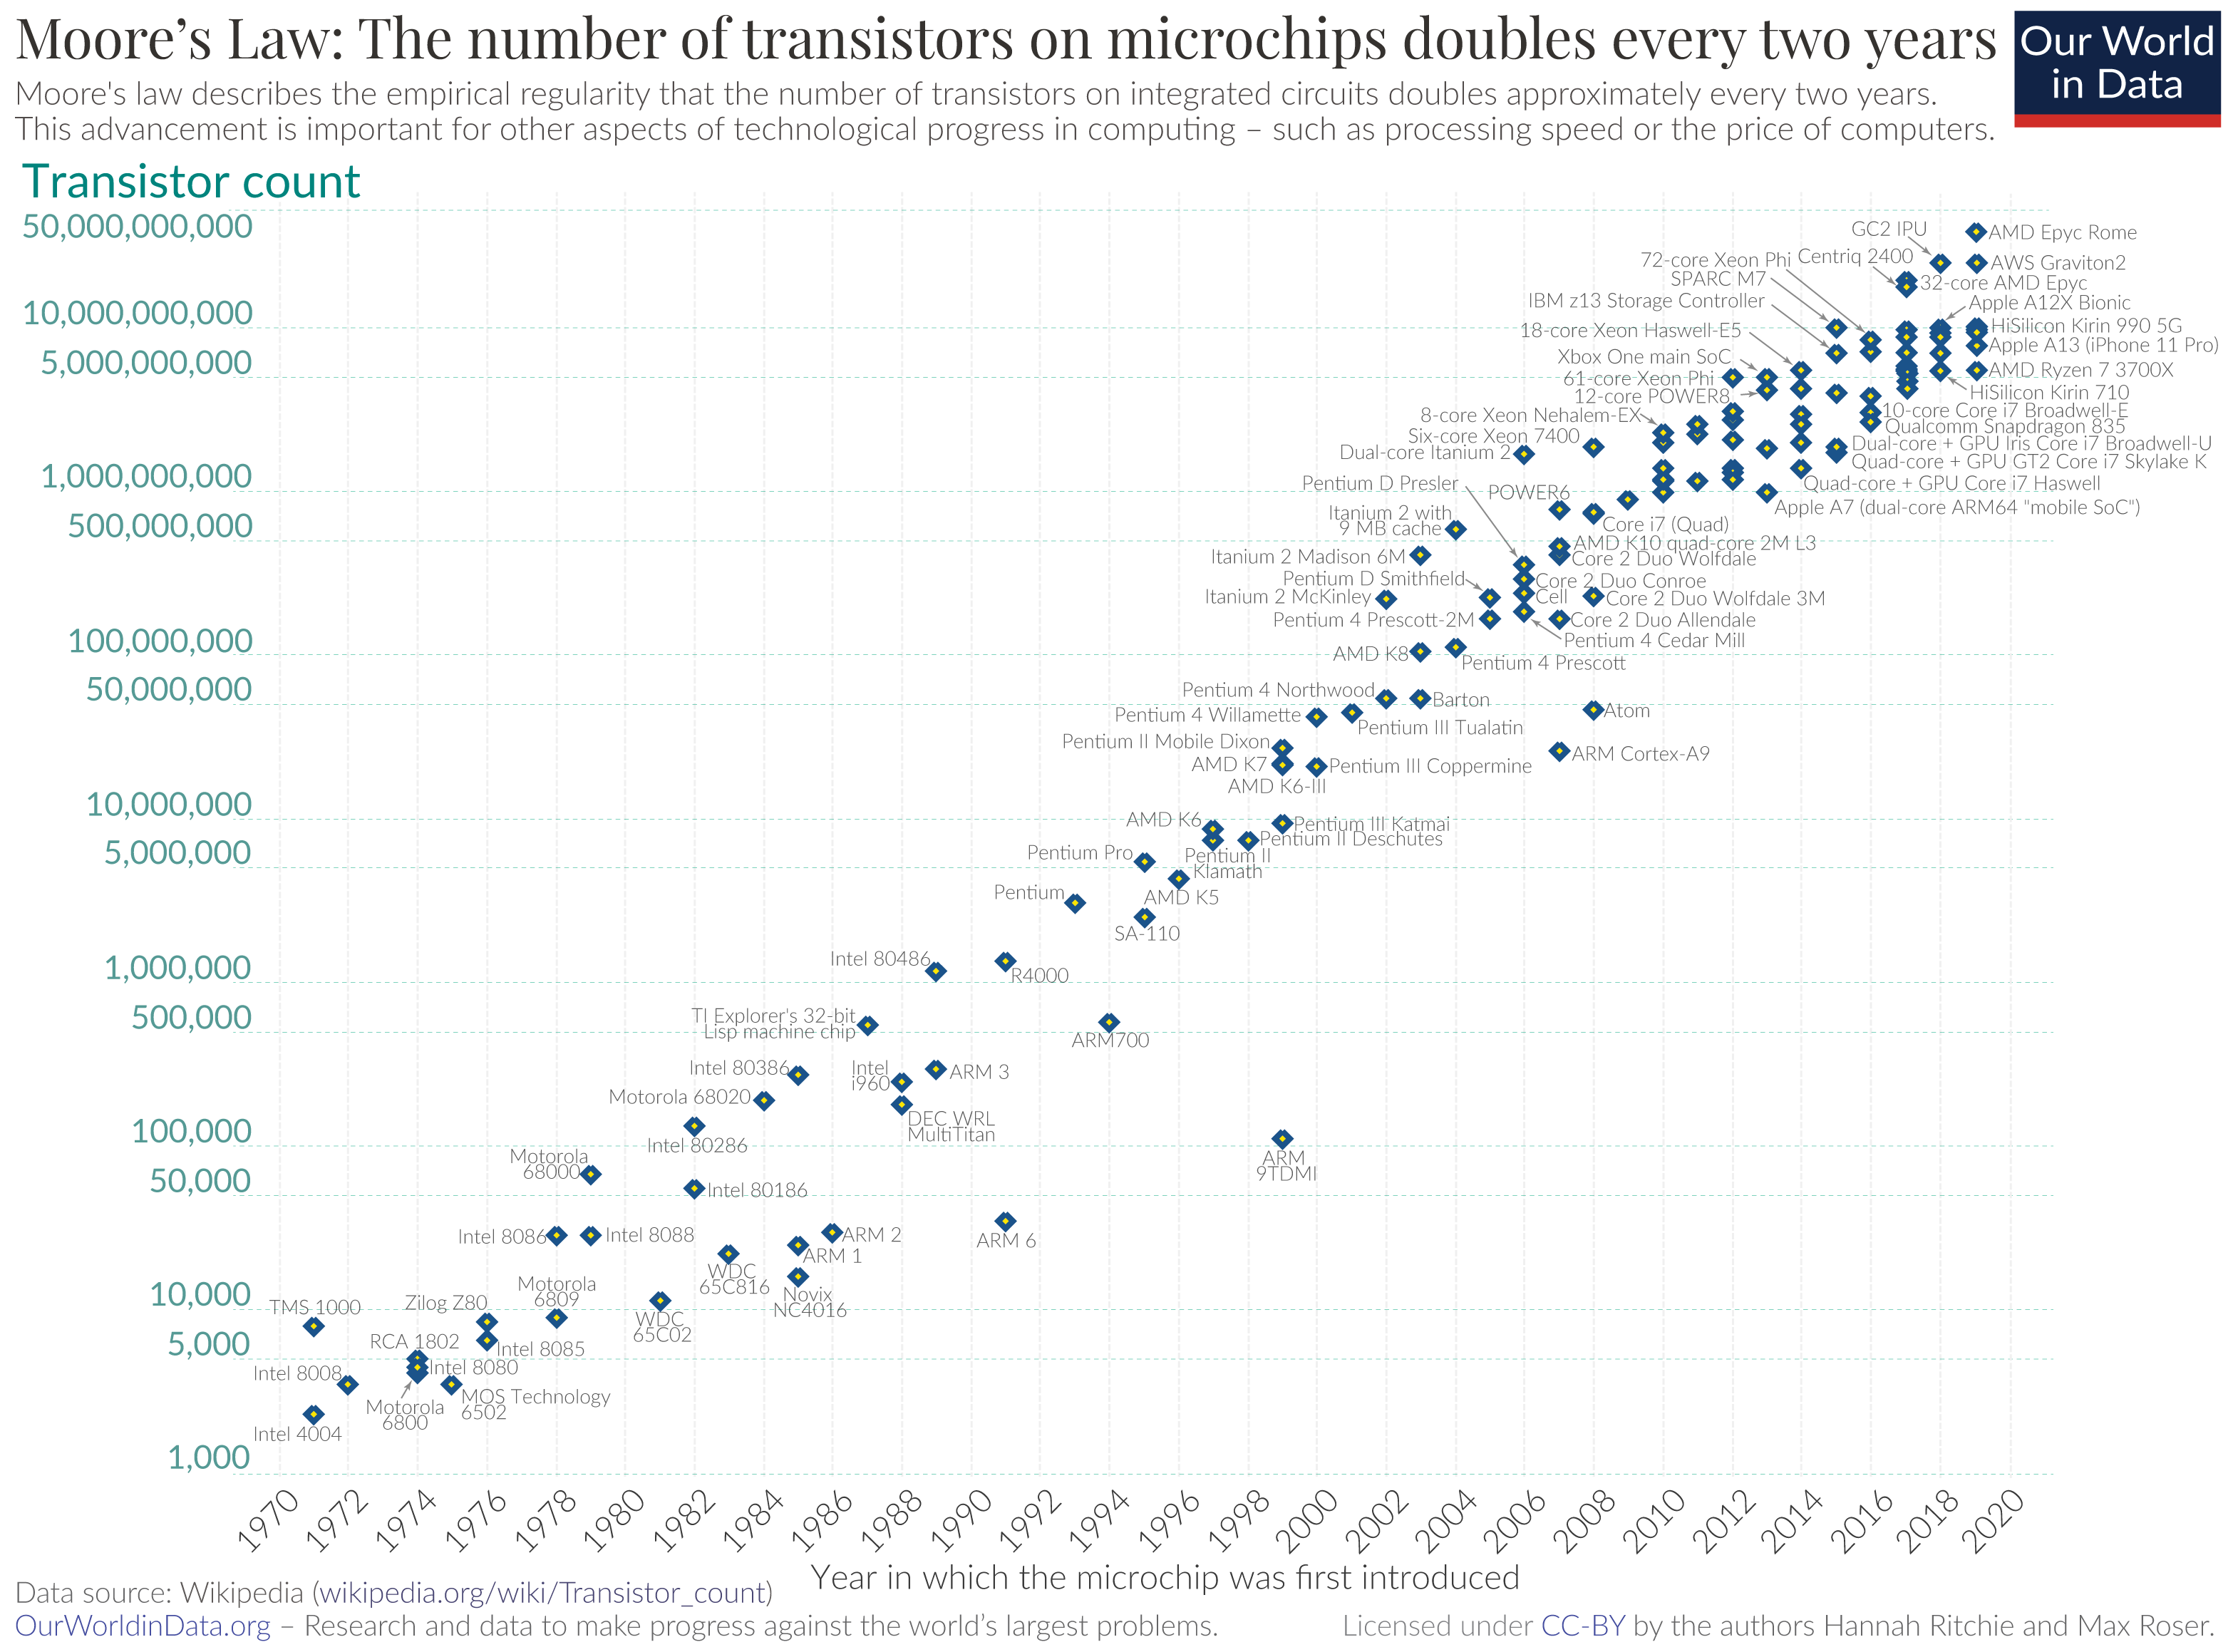
\includegraphics[scale=0.12]{Moore's_Law_Transistor_Count_1970-2020.png}
\end{figure}
\newpage

\subsection{Difference between  Classical and Quantum computing}
\label{subsec: Difference between  Classical and Quantum computing}
\begin{figure}[h]
    \centering
    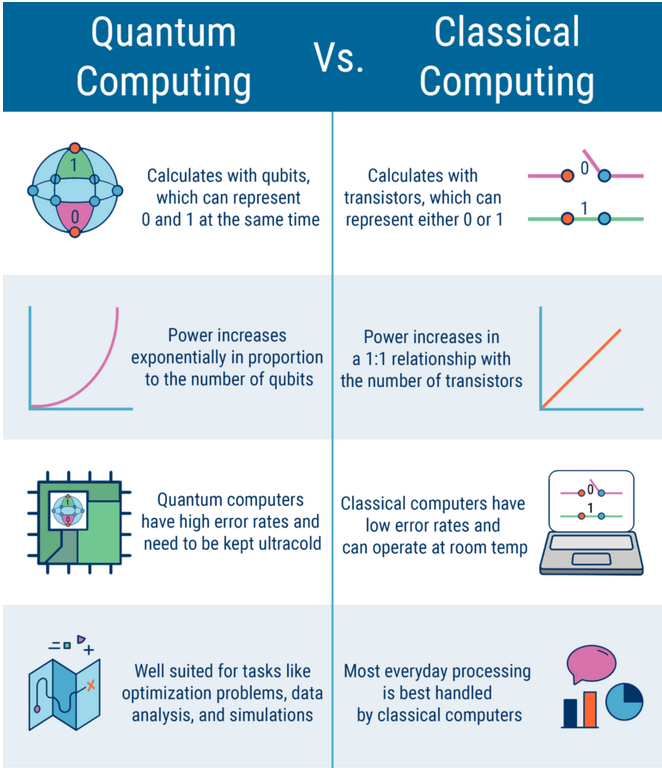
\includegraphics[scale = 0.5]{cc_qc.png}
\end{figure}

\subsection{Quantum superposition}
\label{subsec:Quantum superposition}
Quantum superposition is a fundamental principle of quantum mechanics. It states that, much like waves in classical physics, any two (or more) quantum states can be added together (“superposed”) and the result will be another valid quantum state; and conversely, that every quantum state can be represented as a sum of two or more other distinct states.

\section{Properties of a qubits}
\label{Properties of a qubits}

\subsection{Mathematical representation}
\label{Mathematical representation}
Consider a coin toss. Once the coin is tossed in the air, let's say an invisible cloak, masks the coin.  
Based on this situation, we can store the coin toss result information in this format,
\begin{equation*}
    result = \begin{bmatrix}
        heads \\ tails
    \end{bmatrix} 
\end{equation*}
As the tossed coin is masked by the invisibility cloak, if the result of the coin toss is heads, then this information will be represented in the form,
\begin{equation}
    result(heads) = \ket{0} = \begin{bmatrix}
        heads = 1 \\ tails = 0
    \end{bmatrix} = \begin{bmatrix}
        1 \\ 0
    \end{bmatrix}
\end{equation}
Else, if the result of the coin toss is assumed to be tails, then the information of this result will be stored in the format,
\begin{equation*}
    result(tails) = \ket{1} = \begin{bmatrix}
        heads = 0 \\ tails = 1
    \end{bmatrix} = \begin{bmatrix}
        0 \\ 1 
    \end{bmatrix}
\end{equation*}

\textbf{Note:} There is very particular reason why we use these notations and representation. Based on this type of matrix notation, we can store much information in concise and understandable format.

Now that you have gone through the topics := \hyperref[subsec: Special States]{Special states}, \hyperref[subsec:Schrödinger's cat]{Schrödinger’s cat} and \hyperref[subsec:Qubits!]{Qubits!}, we can apply these concepts for the coin toss problem. So, the information of the overall result, of the coin toss can be represented in the form,
\begin{equation*}
    \text{Total result} = \text{result (heads) + result (tails)} = \ket{0} + \ket{1} = \begin{bmatrix}
        heads = 1 \\ tails = 0
    \end{bmatrix} + \begin{bmatrix}
        heads = 0 \\ tails = 1
    \end{bmatrix}
\end{equation*}

or, simply a quantum superposed state,
\begin{equation}
    \ket{\psi} = \begin{bmatrix}
        heads = 1 \\ tails = 0
    \end{bmatrix} + \begin{bmatrix}
        heads =0 \\ tails =1
    \end{bmatrix} = \begin{bmatrix}
        1 \\ 0 
    \end{bmatrix} + \begin{bmatrix}
        0 \\1
    \end{bmatrix}
\end{equation}
So, now we can say that the result of the coin toss is a superposed state. This information of the coin toss which is represented by the above equation can be referred as 1 qubit.\\
\textbf{Note:} $\ket{\psi}$ is not normalized. You can do it as a small exercise.\\
If the invisibility cloak is unmasked, and I observe the result of the coin toss is heads, then the result of the above equation will be of the form,
\begin{equation*}
    \text{invisibility cloak unmasked}(\ket{\psi}) = \begin{bmatrix}
        heads = 1 \\ tails = 0
    \end{bmatrix} + \cancel{\begin{bmatrix}
        heads =0 \\ tails =1
    \end{bmatrix}} = \begin{bmatrix}
        1 \\ 0 
    \end{bmatrix} + \cancel{\begin{bmatrix}
        0 \\1
    \end{bmatrix}}
\end{equation*}

The act of unmasking the invisibility cloak is called \underline{an act of measurement}.

\subsection{Representation of qubit by Bloch
sphere}
\label{Representation of qubit by Bloch
sphere}
Naturally, a great deal of attention has been given to the ‘meaning’ or ‘interpretation’
that might be attached to superposition states, and of the inherently probabilistic nature of
observations on quantum systems. However, by and large, we shall not concern ourselves
with such discussions. Instead, our intent will be to develop mathematical
and conceptual pictures which are predictive. One picture useful in thinking about qubits is the following geometric representation.

\begin{figure}[h]
    \centering
    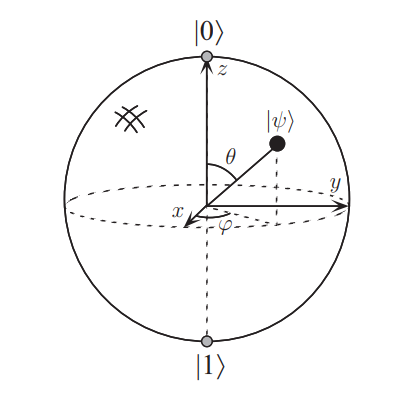
\includegraphics{bloch_sphere.png}
    
\end{figure}
\begin{equation}
    \ket{\psi} = \alpha\ket{0} + \beta\ket{1}
\end{equation}
where, $\alpha$ and $\beta$ are complex numbers and obey the conditions $|\alpha|^{2} + |\beta|^{2} = 1$. For the context of our coin toss experiment, $\alpha = \frac{1}{\sqrt{2}}$ and $\beta = \frac{1}{\sqrt{2}}$ from which we can say what is the probability of the exact result of the coin toss. This can be written in a more generalized and in a more complicated form. But the equation that I am about to give you will be a life changing equation. Behold!
\begin{equation}
    \ket{\psi} = e^{i\gamma}(\cos{\frac{\theta}{2}}\ket{0}+e^{i\phi}\sin{\frac{\theta}{2}}\ket{1})
\end{equation}
where, $\theta,\phi \text{ and } \gamma$ are \underline{real numbers}. Later on we will get to know that the term $e^{i\gamma}$ will not have any observable effects.\\
Thus, the expression will be reduced to,
\begin{equation}
    \ket{\psi} = \cos{\frac{\theta}{2}}\ket{0}+e^{i\phi}\sin{\frac{\theta}{2}}\ket{1}
\end{equation}
The number $\theta$ and $\psi$ define a point on the \underline{unit three-dimensional  sphere}.
The above sphere is often called the \textbf{Bloch sphere}; it provides a useful means of visualizing the state of a single qubit, and often serves as an excellent test-bed for ideas about quantum computation and quantum information.\\

\subsection{Quantum computation}
Changes occurring to a quantum state can be described using the language of \underline{quantum computation}. Analogous to the way a classical computer is built from an electrical circuit
containing wires and logic gates, a quantum computer is built from a \underline{quantum circuit} containing wires and elementary quantum gates to carry around and manipulate the
quantum information. In this section we describe some simple \underline{quantum gates}, and present several example circuits illustrating their application, including a circuit which teleports
qubits!
\section{Quantum Gates}
\label{Quantum Gates}
\subsection{Single qubit gates}
\label{Single qubit gates}
Classical computer circuits consist of wires and logic gates. The wires are used to carry
information around the circuit, while the logic gates perform manipulations of the information, converting it from one form to another. Consider, for example, classical single bit
logic gates.\\
The only non-trivial member of this class is the \textbf{NOT} gate, whose operation is defined by its truth table, in which  $0 \rightarrow 1$  and  $1 \rightarrow 0$ , that is, the $0$ and $1$ states are interchanged.\\
Imagine that we had some process which took the state $\ket{0}$ to the state $\ket{1}$, and vice versa. Such a process would obviously be a good candidate for a quantum analogue to the \textbf{NOT} gate. However, specifying the action of the gate on the states $\ket{0}$ and $\ket{1}$ does not tell us what happens to the superpositions of the states $\ket{0}$ and $\ket{1}$, without further knowledge about the properties of quantum gates. In fact, the quantum \textbf{NOT} gate acts \underline{linearly}, that is, it takes the state 
\begin{equation}
    \alpha\ket{0}+\beta\ket{1}
\end{equation}
to the corresponding state in which the role of 
$\ket{0}$ and $\ket{1}$ have been interchanged,
\begin{equation}
    \alpha\ket{1}+\beta\ket{0}
\end{equation}
\textbf{Note}: It turns out that this linear
behavior is a general property of quantum mechanics, and very well motivated empirically;
moreover, nonlinear behavior can lead to apparent paradoxes such as time travel, faster than-light communication, and violations of the second laws of thermodynamics.\\
There is a convenient way of representing the quantum \textbf{NOT} gate in matrix form,
which follows directly from the linearity of quantum gates. Suppose we define a matrix
$X$ to represent the quantum gate as follows:
\begin{equation}
    X = \begin{bmatrix}
        0 & 1 \\ 1 & 0 
    \end{bmatrix}
\end{equation}
If the quantum state $\alpha\ket{0}+\beta\ket{1}$ is written in a vector notation as
\begin{equation}
\begin{bmatrix}
    \alpha \\ \beta
\end{bmatrix} 
\end{equation},
with the top entry corresponding to the amplitude for $\ket{0}$ and the bottom entry the amplitude for $\ket{1}$, then the corresponding output from the quantum \textbf{NOT} gate is 
\begin{equation}
    X\begin{bmatrix}
        \alpha \\ \beta
    \end{bmatrix} = \begin{bmatrix}
        \beta \\ \alpha
    \end{bmatrix}
\end{equation}
Notice that the action of the gate is to take the state $\ket{0}$ and replace it by the state
corresponding to the first column of the matrix $X$. Similarly, the state $\ket{1}$ is replaced by the state corresponding to the second column of the matrix $X$. So quantum gates on a single qubit can be described by $2 \times 2$ matrices.\\
Are there
any constraints on what matrices may be used as quantum gates?\\
It turns out that there are.\\
Recall that the normalization condition requires $|\alpha|^{2}+|\beta|^{2} = 1$ for a quantum state
$\alpha\ket{0} + \beta\ket{1}$. This must also be true of the quantum state, $\ket{\psi'}=\alpha'\ket{0} + \beta'\ket{1}$ after the
gate has acted. \\
It turns out that the appropriate condition on the matrix representing the gate is that the matrix U describing the single qubit gate be unitary, that is $U^{\dagger}U = I$,
where $U^{\dagger}$ is the adjoint of U (obtained by transposing and then complex conjugating U), and $I$ is the $2 \times 2$ identity matrix. For example, for the gate, it is easy to
verify that $X^{\dagger}X=I$.\\
Amazingly, this unitarity constraint is the only constraint on quantum gates. Any unitary matrix specifies a valid quantum gate! The interesting implication is that in contrast to the classical case, where only one non-trivial single bit gate exists—the \textbf{NOT} gate-there are many non-trivial single qubit gates. Two important one which we need to study is $Z$ gate:
\begin{equation}
    Z \equiv \begin{bmatrix}
        1 & 0 \\ 0 & -1
    \end{bmatrix}
\end{equation}
which leaves $\ket{0}$ unchanged, and flips the sign of $\ket{1}$ to give $-\ket{1}$, and the \textbf{Hadamard} gate,
\begin{equation}
    H \equiv \frac{1}{\sqrt{2}}\begin{bmatrix}
        1 & 1 \\ 1 & -1
    \end{bmatrix}
\end{equation}

\vspace{0.2cm}

\begin{center}
    \begin{quantikz}
\lstick{$\alpha\ket{0}+\beta\ket{1}$\\initial state} & \qw & \gate{X} & \qw 
    & \rstick{$\alpha\ket{1} + \beta\ket{0}$} \qw
\end{quantikz}
\end{center}

\vspace{0.2cm}

\begin{center}
    \begin{quantikz}
\lstick{$\alpha\ket{0}+\beta\ket{1}$\\initial state} & \qw & \gate{Z} & \qw 
    & \rstick{$\alpha\ket{0} - \beta\ket{1}$} \qw
\end{quantikz}
\end{center}

\vspace{0.2cm}

\begin{center}
    \begin{quantikz}
\lstick{$\alpha\ket{0}+\beta\ket{1}$\\initial state} & \qw & \gate{H} & \qw 
    & \rstick{$\alpha\frac{\ket{0}+\ket{1}}{\sqrt{2}} + \beta \frac{\ket{0}-\ket{1}}{\sqrt{2}} $}
    \qw
\end{quantikz}
\end{center}

Recalling the Pauli matrices, we treat these matrices as gates.

\begin{equation}
    \sigma_{x} = \begin{bmatrix}
        0 & 1 \\ 1 & 0
    \end{bmatrix},\hspace{0.15cm} 
    \sigma_{y} = \begin{bmatrix}
        0 & -i \\ +i & 0
    \end{bmatrix} \text{and} \hspace{0.15cm}
    \sigma_{z} = \begin{bmatrix}
        1 & 0 \\ 0 & -1
    \end{bmatrix}
\end{equation}

Similar to the $X$-gate, which is analogous to the classical \textbf{NOT}-gate. The $\sigma_{y}$ is the $Y$-gate and $\sigma_{z}$ is the $Z$-gate.\\
To understand the above huge load of information, let us understand in summarized way.
\newpage
\subsubsection{Quantum Gates Basic}
\label{subsubsec: Quantum Gates Basic}
\textbf{The Pauli Z-gate Operation}
\begin{itemize}
    \item The state vector of a qubit can be represented as two orthogonal vectors.
    \item The state vector of a qubit can be represented as two orthogonal vectors. 
$\ket{0} = \begin{bmatrix} 1 \\ 0\end{bmatrix}$ and 
$\ket{1} = \begin{bmatrix} 0 \\ 1 \end{bmatrix}$.
    \item  Represented by Pauli Z-matrix 
$Z = \begin{bmatrix} 1 & 0 \\ 0 & -1 \end{bmatrix}$.
    \item  It's a phase shift gate, sometime called \textbf{phase-flip}. Rotating around the Z-axis of the Bloch sphere by $\pi$ radians.
    \item It leaves the basis state $\ket{0}$ unchanged and maps to $\ket{1}$ to $-\ket{1}$.
\end{itemize}
\textbf{Introduction to Hadamard $H$ gate}
\begin{itemize}
    \item using only the Pauli-gates, we are now able to get only the states $\ket{0}$ and $\ket{1}$, similar to classical bit $1$ or $0$ ('ON' or 'OFF').
    \item To harness the power of Qubits, we must move away from the poles of the Bloch sphere and create a superposition.
    \item Represented by the Hadamard matrix 
$H = \frac{1}{\sqrt{2}}\begin{bmatrix} 1 & 1 \\ 1 & -1 \end{bmatrix}$.
     \item It will transform the state of the qubit between the $X$ and $Z$ bases, as a rotation around the Bloch vectors [1,0,1] (the line between the X and Z axes)
    \item Change the state $\ket{0}$ to $\ket{+}$ and $\ket{1}$ to $\ket{-}$,\\
    \vspace{0.2cm}
$H\ket{0} = \ket{+} = \frac{1}{\sqrt{2}}\begin{bmatrix}1 \\1 \end{bmatrix}$ \\
$H\ket{1} = \ket{-} = \frac{1}{\sqrt{2}}\begin{bmatrix}1 \\-1 \end{bmatrix}$
\end{itemize}
\newpage
\large{\textbf{$R\phi$-gate}}
\begin{itemize}
    \item Using a number parameter ($\phi$) to tell it to performs a rotation of $\phi$ around the Z-axis direction. (Where $\phi$ is a real number)
    \item It is also called as $RZ$-gate.
    \item The transformation matrix for $R\phi$ gate is 
    $R_{\phi} = \begin{bmatrix} 1 & 0 \\ 0 & e^{i\phi} \end{bmatrix}$.
    \item From $R\phi$-gate we get I, Z, S and T gates.
\end{itemize}       
\textbf{The $S$-gate and $S^{\dagger}$-gate}
\begin{itemize}
    \item S-gate is a $R\phi$ gate with $\phi = \frac{\pi}{2}$.
    \item S-gate is not its own inverse.
    \item Two S-gate together will give only a Z-gate equivalent.
    \item The $S^{\dagger}$ gate is a $R\phi$ with $\phi = \frac{-\pi}{2}$.
    \item The transformation matrix for $S$ and $S^{\dagger}$ are 
$S = \begin{bmatrix}1&0\\ 0 & e^{\frac{i\pi}{2}}\end{bmatrix}$,\\
$S^{\dagger} = \begin{bmatrix}1&0\\ 0 & e^{\frac{-i\pi}{2}}\end{bmatrix}$.
\end{itemize}
\textbf{The $T$-gate and $T^{\dagger}$-gate}
\begin{itemize}
    \item T-gate is a $R\phi$ gate with $\phi = \frac{\pi}{4}$.
    \item Two T-gate together will give only a Z-gate equivalent.
    \item The $T^{\dagger}$ gate is a $R\phi$ with $\phi = \frac{-\pi}{4}$.
    \item The transformation matrix for $T$ and $T^{\dagger}$ are 
$T = \begin{bmatrix}1&0\\ 0 & e^{\frac{i\pi}{4}}\end{bmatrix}$,
$T^{\dagger} = \begin{bmatrix}1&0\\ 0 & e^{\frac{-i\pi}{4}}\end{bmatrix}$
\end{itemize}
\newpage
\textbf{General $U$-gate ($U_{3}$, $U_{2}$, $U_{1}$)}\\
\begin{itemize}
    \item  $U_{3}$ gate is the generalized version of gates like X, Y, H gates.
    \item It's a parameterized form of 
$U_{3}(\theta,\phi,\lambda) = 
\begin{bmatrix}\cos(\frac{\theta}{2}) & -e^{i\lambda}\sin(\frac{\theta}{2} )\\ \\ e^{i\phi}\sin(\frac{\theta}{2})& e^{i(\lambda+\phi)}\cos(\frac{\theta}{2})
\end{bmatrix} $
    \item Also there are $U_{2}$ and $U_{1}$ gates which are also $U_{3}$ gate with $\theta = \frac{\pi}{2}$, $\theta = 0$ and $\phi = 0$ respectively.\\
$U_{3}(\frac{\pi}{2},\phi,\lambda) = \frac{1}{\sqrt{2}}
\begin{bmatrix}1 & -e^{i\lambda}\\ \\e^{i\phi}& e^{i(\lambda+\phi)}
\end{bmatrix} $\\
\vspace{0.2cm}
$U_{3}(0,0,\lambda) = 
\begin{bmatrix}1 & 0\\ 0 & e^{i(\lambda)}
\end{bmatrix} $

\end{itemize}

\subsection{Multi Qubit System}
\label{subsec:Multi Qubit System}

\subsubsection{Multi-Qubit gates}
\begin{itemize}
    \item Single qubits offer no computational advantage. Interaction between qubits is the true power of quantum computing.
    \item Gates directly implemented in hardware will act only on one or two  qubits. With those gates, it is possible to build any other gate.
    \item A single bit has two possible states, $0$ and $1$.
    \item A qubit has two states, $\ket{0}$ and $\ket{1}$ and complex amplitude. Two bits have four possible states: $00$, $01$, $10$ and $11$.
    \item Like that, two qubits requires four complex amplitudes to represent its states.
    \item For the two separates qubits, we can describe their collective state using the tensor product:
    \begin{equation*}
        \ket{a} = \begin{bmatrix}
            a_{o} \\ a_{1}
        \end{bmatrix}, \hspace{0.2cm} \ket{b} = \begin{bmatrix}
            b_{o} \\ b_{1}
        \end{bmatrix} 
    \end{equation*}
    \vspace{0.1cm}
    \begin{equation}
        \ket{ba} = \ket{b} \otimes \ket{a} = \begin{bmatrix}
            b_{o} \times \begin{bmatrix}
            a_{o} \\ a_{1}
        \end{bmatrix} \\ \\ b_{1} \times \begin{bmatrix}
            a_{o} \\ a_{1}
        \end{bmatrix}
        \end{bmatrix} = \begin{bmatrix}
            b_{o}a_{o}\\b_{o}a_{1}\\b_{1}a_{o}\\b_{1}a_{1}
        \end{bmatrix}
    \end{equation}
    \item Can you guess how many complex amplitudes are required to represent a three qubit state ?
\end{itemize}

\subsubsection{Single vs Multi Qubits}

\begin{itemize}
    \item Generally, if we have \underline{$n$ qubits}, we will need to keep track of \underline{$2^{n}$ complex amplitudes} to describe their states.
    \item A modern classical computer can easily simulate a general quantum state of around $20$ qubits.
    \item \textbf{Example:} If only one gate is applied to a $2$ qubit circuit, we can do its tensor product with the identity matrix.
    \begin{equation*}
        X \otimes I = \begin{bmatrix}
            0 & 1 \\ 1 & 0
        \end{bmatrix}\otimes\begin{bmatrix}
            1 & 0 \\ 0 & 1
        \end{bmatrix} = \begin{bmatrix}
            0&0&1&0 \\ 0&0&0&1 \\ 1&0&0&0 \\ 0&1&0&0
        \end{bmatrix} = \begin{bmatrix}
            0 & I \\ I & 0
        \end{bmatrix}
    \end{equation*}
\end{itemize}

\subsubsection{Multiple Qubits and \textbf{CNOT} Gate}

\begin{itemize}
    \item Performs a $X$-gate on the second qubit (called as \underline{target}), if the states of the first qubit (called as \underline{CONTROL}) is $\ket{1}$.
    \begin{center}
         \begin{quantikz}
        \lstick{$\ket{q_{o}}$} & \ctrl{1} & \qw \\
        \lstick{$\ket{q_{1}}$} & \targ{} & \qw
    \end{quantikz}
    \end{center}
    
    
    
    \item Truth table of \textbf{CNOT} Gate when qubits are not \underline{entangled} (Not in superposition).

    \begin{table}[h]
        \centering
        \begin{tabular}{|c|c|}
        \hline
        Input (t,c) & Output (t,c)\\
        \hline
           00  & 00\\
           01 & 11\\
           10 & 10\\
           11 & 01\\
           \hline
        \end{tabular}
    \end{table}

    \item For the \textbf{CNOT} gate when the qubits are in entangled state, we change the basis states from $\ket{0}$,$\ket{1}$ to $\ket{+}$ and $\ket{-}$. By applying, the Hadamard gate to $\ket{0}$ and $\ket{1}$, the basis states changes to $\ket{+}$ and $\ket{-}$.

    \item Applying the \textbf{CNOT} gate to the $\ket{+}$ end  $\ket{-}$ states, say
    \begin{equation*}
        CNOT\ket{-+} = \frac{1}{2}(\ket{00}-\ket{01}-\ket{10}+\ket{11}) = \ket{--}
    \end{equation*}
   \item State of the target qubit unchanged, but control qubit changes.
   
   \item \textbf{CNOT} swaps the amplitudes of $\ket{01}$ and $\ket{11}$.
   
   \item It has $25\%$ probability of being measured in the states $\ket{00}$,$\ket{01}$,$\ket{10}$, and
$\ket{11}$.
    \item The Bloch sphere shows both the same because \textbf{CNOT} only interchanges the amplitudes of $\ket{01}$ and $\ket{11}$.
    \begin{table}[h]
        
        \begin{tabular}{c|c|c|c|c}
        \hline
        Initial States & Computational Basis & Apply operator & Resulting basis & Final state \\
        \hline 
            \vspace{0.3cm}
            $\ket{++}$ & $\frac{1}{2}(\ket{00}+\ket{01}+\ket{10}+\ket{11})$ & CNOT & $\frac{1}{2}(\ket{00}+\ket{01}+\ket{11}+\ket{10})$ & $\ket{--}$ \\
            \vspace{0.3cm}\
            $\ket{+-}$ & $\frac{1}{2}(\ket{00}-\ket{01}+\ket{10}-\ket{11})$ & CNOT & $\frac{1}{2}(\ket{00}-\ket{01}+\ket{11}-\ket{10})$ & $\ket{--}$ \\
            \vspace{0.2cm}
            $\ket{-+}$ & $\frac{1}{2}(\ket{00}+\ket{01}-\ket{10}-\ket{11})$ & CNOT & $\frac{1}{2}(\ket{00}+\ket{01}-\ket{11}-\ket{10})$ & $\ket{-+}$ \\
            \vspace{0.2cm}
            $\ket{--}$ & $\frac{1}{2}(\ket{00}-\ket{01}-\ket{10}+\ket{11})$ & CNOT & $\frac{1}{2}(\ket{00}-\ket{01}-\ket{11}+\ket{10})$ & $\ket{++}$ \\
             
        \hline
             
        \end{tabular}
    \end{table}
    
    
\end{itemize}
\newpage
\subsubsection{Controlled Z gate}
\begin{itemize}
    \item Just like \textbf{CNOT} applies $X$ to \underline{target} whenever \underline{control} is 1.
    \item Like \textbf{CZ} applies $Z$ to target whenever \underline{control} is 1.
    \begin{table}[h]
        \centering
        \begin{tabular}{|c|c|}
        \hline
        Input (t,c) & Output (t,c)\\
        \hline
           $\ket{00}$  & $\ket{00}$\\
           $\ket{01}$  & $\ket{01}$\\
           $\ket{10}$  & $\ket{10}$\\
           $\ket{11}$  & $-\ket{11}$\\
           \hline
        \end{tabular}
    \end{table}
\end{itemize}

\subsubsection{SWAP Gate}
\begin{itemize}
    \item \textbf{SWAP} gate is used to move the state between two qubits.
    \item The \textbf{SWAP} gate is represented as,
    \begin{center}
        \begin{quantikz}
        \lstick{$\ket{0}$} & \gate{H} & \swap{1} & \qw \\
        \lstick{$\ket{0}$} &\qw & \targX{} & \qw 
    \end{quantikz}
    \end{center}
    \item In real Quantum computer, \underline{the only two-qubit gate that can be directly applied is the CNOT gate.}
    \item So in order to get SWAP gate, we have to create identical circuit using CNOT gates.
    
\end{itemize}
\newpage
\subsubsection{Toffoli gate}
\begin{itemize}
    \item The Toffoli gate is a three qubit gate with two control and one target. It \underline{performs an $X$ on the target only if both controls are in the state $\ket{1}$}.
    \item It is controlled-controlled-NOT, and is also called the \textbf{CCX} gate.
    \item The truth table of the Toffoli gate is given by,
    \begin{figure}[h]
        \centering
        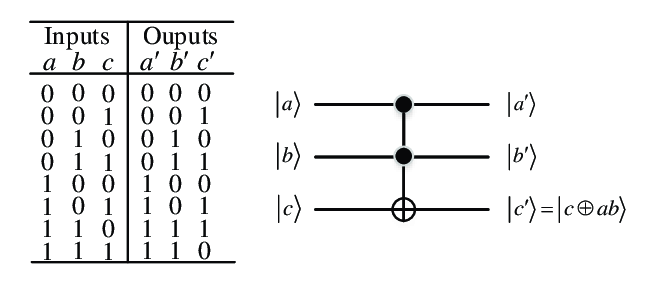
\includegraphics[scale=0.7]{Truth-table-and-quantum-circuit-of-Toffoli-gate.png}
    \end{figure}
\end{itemize}

\newpage
\section{WARNING!}
This document is more of a reference material. Detailed information is not provided in this document, as it requires rigorous mathematics. Please make your own notes so that you are comfortable with the concepts and notations. Apart from this document, the below listed sources are good options:
\begin{itemize}
    \item \href{https://www.youtube.com/watch?v=ZuvCUU2jD30&list=PLxhaPrr4aQ9lnBEOoy7r6KNlrTG_obLgr}{Quantum Computing lecture series}
    \item \href{https://www.youtube.com/watch?v=rtI5wRyHpTg}{Moore's Law }
    \item \href{https://www.youtube.com/watch?v=JRIPV0dPAd4}{A Beginner's Guide to Quantum Computing}
    
\end{itemize}
\end{document}
